\documentclass[12pt, letterpaper]{article}
\usepackage[utf8]{inputenc}
\usepackage{indentfirst}
\usepackage{graphicx}

\graphicspath{ {images/} }

\title{Trabalho 5 - MC920}
\author{Rian Radeck Santos Costa - 187793}
\date{02 de Dezembro de 2022}

\begin{document}

\maketitle
\newpage

\section{Objetivo}
		Detectar mudanças entre frames de um vídeo e destacá-las para o usuário. 

		Obviamente os vídeos apresentados pelo meu programa têm nuâncias e origem diferentes e acredito que os parâmetros usados no código não sejam os ótimos para todos os casos, mas tentei fazer com que ficasse razoável em todos os exemplos.
		\subsection{Plano de ação}
		\begin{enumerate}
			\item{Transformar a imagem para uma imagem em tons de cinza.}
			\item{Calcular a diferença entre o frame atual e o ultimo gerado.}
			\item{Na diferença, separar objeto de fundo.}
			\item{Contornar objetos relevantes (de área grande suficiente) com retângulos.}
		\end{enumerate}

\section{Implementação}
	Para obter o frame passado apenas salvei ele na variável ``last'' no final do loop e pulo o loop no primeiro frame.
	\subsection{Tons de Cinza}
		Para trasnfomar um frame em tons de cinza apenas utilizei a função ``cv.cvtColor(frame, cv.COLOR\_BGR2GRAY)'' do OpenCV.
	\subsection{Cálculo da Diferença}
		Para calcular a diferença utilizei a função ``np.abs(frame - last)'' do numpy. Além disso, precisamos notar que apenas subtrair frame e last pode causar um underflow no tipo uint8, então precisamos converter essa operação para um tipo que suporte valores negativos, sendo assim nossa função correta seria ``diff = np.abs(gray.astype("int16") - last.astype("int16")).astype("uint8")''.
	\subsection{Detecção de Objetos}
		Para separar objeto de fundo, foram utilizadas técnicas de limiarização, suavização e dilatação na imagem original (diferença). Utilizei sempre as funções do OpenCV, os parâmetros que melhor se encaixaram no meu exemplo estão descritos no código (linhas 19 à 21). Para a dilatação escolhi uma dilatação elíptica (no caso circular) para dilatação em todas as direções, mas é claro que se soubermos a direção principal da movimentação de nosso vídeo podemos aumentar um dos eixos da elipse. Por exemplo, estamos querendo detectar carros passando em uma estrada e estamos gravando a beira dela de tal forma que os carros passam da direita para a esquerda, em um movimento horizontal, sendo assim poderiamos deixar o eixo horizontal da elipse maior.
	\subsection{Contorno dos Objetos}
		Após descobrir vários objtos apenas passei eles para a função ``cv.findContours(img, cv.RETR\_TREE, cv.CHAIN\_APPROX\_SIMPLE)'' para descobrir seus contornos. Depois iterei por cada contorno verificando se ele era relevante e encontrando seu retângulo de limites com a função ``cv.boundingRect(contour)''. Depois disso apenas desenhei o retângulo juntamente co a imagem original com a função ``cv.rectangle()''. Obs.: ser relevante depende da resolução da imagem.

\newpage
\section{Imagens}
	\begin{figure}[h]
        \centering
        
\includegraphics[width=0.4\textwidth]{diff.png}
        \\{Diferença DVD}
    \end{figure}

    \begin{figure}[h]
        \centering
        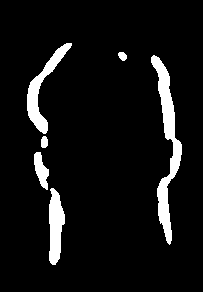
\includegraphics[width=0.4\textwidth]{objects.png}
        \\{Objetos Rian}
    \end{figure}

    \begin{figure}[h]
        \centering
        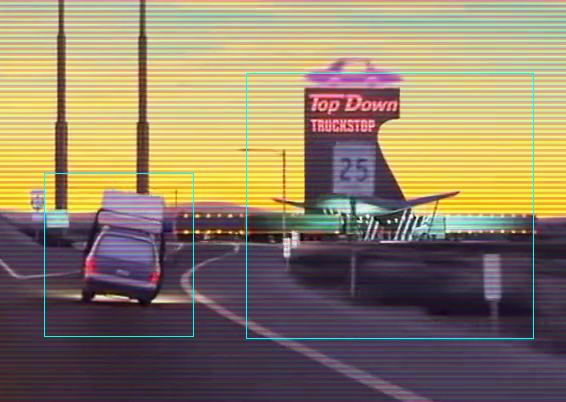
\includegraphics[width=1\textwidth]{rectangles.png}
        \\{Destacados Carros}
    \end{figure}



\end{document}